The term "vacuum" has distinct meanings across classical physics, quantum field theory, and general relativity. In classical physics, vacuum refers to the absence of material particles: a region of space devoid of atoms, molecules, or macroscopic matter. The classical vacuum is an empty stage on which forces act.

In quantum field theory (QFT), the notion of vacuum acquires a different character. Here, fields — not particles — constitute the primary entities. The vacuum is defined as the ground state of all quantum fields: the configuration of lowest possible energy consistent with the commutation relations and field dynamics. Even when no particles are present, quantum fields fluctuate around their minima, giving rise to nonzero vacuum expectation values for certain observables. These fluctuations are not artifacts of measurement or disturbance; they are features of the quantum equations themselves. Crucially, in flat Minkowski spacetime and for inertial observers, the vacuum is Lorentz invariant: no preferred direction or frame exists, and the absence of particles is an absolute property relative to all inertial frames.

However, in general relativity (GR), spacetime is no longer a fixed, flat background. It becomes a dynamical entity whose curvature interacts with matter and energy. The introduction of curved spacetime disrupts the global symmetries that underlie the inertial vacuum of QFT. In regions of strong gravitational fields or global curvature, there is generally no unique, globally defined vacuum state. Instead, the concept of vacuum becomes observer-dependent. Different families of observers may disagree about whether a given region of spacetime is populated by particles. This relativity of the vacuum arises because the definition of positive frequency modes — those corresponding to particle excitations — depends on the choice of time coordinate, which itself is tied to the observer's worldline. Consequently, what one observer identifies as an empty vacuum, another observer may interpret as a state containing particles, momentum, or thermal radiation.

The transition from a universal to an observer-relative vacuum marks a change in physical ontology. It reflects the interplay between quantum mechanics and the geometric nature of general relativity, a relationship that becomes central in contexts such as black hole thermodynamics, early-universe cosmology, and accelerating reference frames.

In quantum field theory, the notion of a particle is defined relative to specific mode decompositions of the fields. In flat Minkowski spacetime, the Poincaré symmetry provides a natural criterion for identifying positive-frequency solutions to the field equations. These modes, typically plane waves with time dependence $e^{-i\omega t}$ and $\omega > 0$, underpin the construction of creation and annihilation operators. The vacuum state is then characterized as the state annihilated by all annihilation operators, and particles are defined as excitations above this vacuum.

A Killing vector field is a vector field which is invariant under the flow of the group of isometries of the manifold. In Minkowski spacetime, the group of isometries is the Poincaré group, which includes translations, rotations, and boosts. The timelike Killing vector field is the generator of time translations.

The existence of a global timelike Killing vector field in Minkowski spacetime ensures that the decomposition into positive and negative frequencies is observer-independent among inertial observers. This makes the notion of particle number absolute: all inertial observers agree on the absence or presence of particles.

However, when considering non-inertial observers or curved spacetimes, this symmetry is broken. In general spacetimes, no global timelike Killing vector field exists. As a result, the separation of field solutions into positive and negative frequencies becomes observer-dependent. The lack of a preferred global time coordinate means that different observers, following different trajectories or employing different coordinate systems, naturally define particles in different ways.

Mathematically, if one observer expands the field $\hat{\phi}(x)$ in terms of a basis of modes $\{f_i(x)\}$, while another observer uses a different basis $\{g_j(x)\}$, the two expansions are related by a Bogoliubov transformation. This transformation mixes creation and annihilation operators, leading to the possibility that the vacuum state for one observer appears populated with particles to another. Specifically, if the Bogoliubov coefficients $\beta_{ij}$ are nonzero, the expected particle number for the second observer, measured in the first observer's vacuum, is nonzero:
\[
\langle 0_f | \hat{N}_g | 0_f \rangle = \sum_j |\beta_{ij}|^2.
\]

Understanding this observer dependence requires abandoning classical intuition that physical quantities such as particle number are absolute.

The Unruh effect occurs in flat Minkowski spacetime. An inertial observer perceives the vacuum as entirely empty, while an observer undergoing uniform acceleration through the same region perceives a thermal bath of particles with temperature $T_U = \hbar a/(2\pi c k_B)$, where $a$ is the proper acceleration. The accelerating observer follows hyperbolic trajectories and adopts Rindler coordinates, which slice spacetime differently than inertial coordinates. This change in slicing transforms the division of field modes into positive and negative frequencies, converting the inertial vacuum into a mixed thermal state.

Hawking radiation arises near black hole event horizons. An observer falling freely across the horizon encounters no particles — the vacuum appears empty. Yet a distant stationary observer perceives thermal radiation emanating from the black hole with temperature $T_H = \hbar c^3/(8\pi G M k_B)$, where $M$ is the black hole mass. The horizon itself acts as a boundary separating causally disconnected regions. Field modes straddling this boundary undergo a Bogoliubov transformation, generating particle pairs from the perspective of the external observer while the infalling observer experiences only vacuum.

Cosmological particle production occurs in expanding spacetimes described by Friedmann-Lemaître-Robertson-Walker metrics. As the universe expands, the stretching of spatial geometry changes the mode structure of quantum fields. Field modes that begin inside the horizon can be stretched beyond the horizon radius during rapid expansion. An observer comoving with the expansion defines particles relative to modes adapted to the time-dependent metric, while an observer at a different epoch or in a different region uses a different decomposition. Quantum fluctuations in the early universe, amplified by this mechanism, seed the temperature anisotropies observed in the cosmic microwave background.

The dynamical Casimir effect generates particles through time-dependent boundary conditions. In the standard Casimir effect, static conducting plates modify the vacuum energy of the electromagnetic field. When the plates accelerate or their separation oscillates, the changing boundary conditions parametrically amplify vacuum fluctuations, producing real photons. An observer at rest relative to the stationary cavity perceives vacuum, while an observer using coordinates adapted to the time-varying geometry detects photons. Laboratory realizations use superconducting circuits with time-modulated boundary conditions, producing measurable photon creation from vacuum.

\newpage
\vspace{50em}
\begin{table}[ht]
\centering
\footnotesize
\renewcommand{\arraystretch}{1.3}
\setlength{\tabcolsep}{3pt}
\begin{tabular}{|>{\centering\arraybackslash}m{2.0cm}|
                >{\centering\arraybackslash}m{2.2cm}|
                >{\centering\arraybackslash}m{2.2cm}|
                >{\centering\arraybackslash}m{2.2cm}|
                >{\centering\arraybackslash}m{2.2cm}|
                >{\centering\arraybackslash}m{2.2cm}|}
\hline
\textbf{Feature} & \textbf{Unruh Effect} & \textbf{Hawking Radiation} & \textbf{Cosmological Particle Creation} & \textbf{Schwinger Effect} & \textbf{Dynamical Casimir Effect} \\
\hline
\textbf{Physical Context} & Uniform acceleration in flat spacetime & Black hole event horizon & Expanding FLRW universe & Strong external electric field & Time-dependent boundary conditions \\
\hline
\textbf{Primary Mechanism} & Bogoliubov transformation (Minkowski $\leftrightarrow$ Rindler) & Horizon mode mismatch and equivalence principle & Mode stretching and horizon crossing & Vacuum instability via tunneling & Parametric amplification of vacuum fluctuations \\
\hline
\textbf{Key Dependence} & Proper acceleration $a$ & Black hole mass $M$, surface gravity & Hubble rate $H$, coupling strength & Electric field strength $E$ & Modulation frequency and boundary speed \\
\hline
\textbf{Characteristic Scale / Formula} & $T_U = \dfrac{\hbar a}{2\pi c k_B}$ & $T_H = \dfrac{\hbar c^3}{8\pi G M k_B}$ & Particle density $\propto H^2$ & $\Gamma \propto \exp\left(-\dfrac{\pi E_c}{E}\right)$ & Photon production peaks at $\omega_{\text{mod}} \approx 2\omega_{\text{cav}}$ \\
\hline
\textbf{Experimental Probes} & Analogues: BECs, trapped ions, superconducting circuits & Analogues (BECs, fluids); black hole thermodynamics & CMB anisotropies, primordial fluctuations & High-intensity lasers, graphene lattices & SQUID-based circuits, modulated cavities \\
\hline
\end{tabular}
\caption*{
\centering
\textbf{Table:} Comparative overview of observer-dependent vacuum phenomena. Each column represents a distinct physical context in which the concept of vacuum, and thus of particle content, becomes relative to the observer’s state of motion or horizon access.
}
\end{table}
\newpage
\vspace{2em}
\begin{center}
    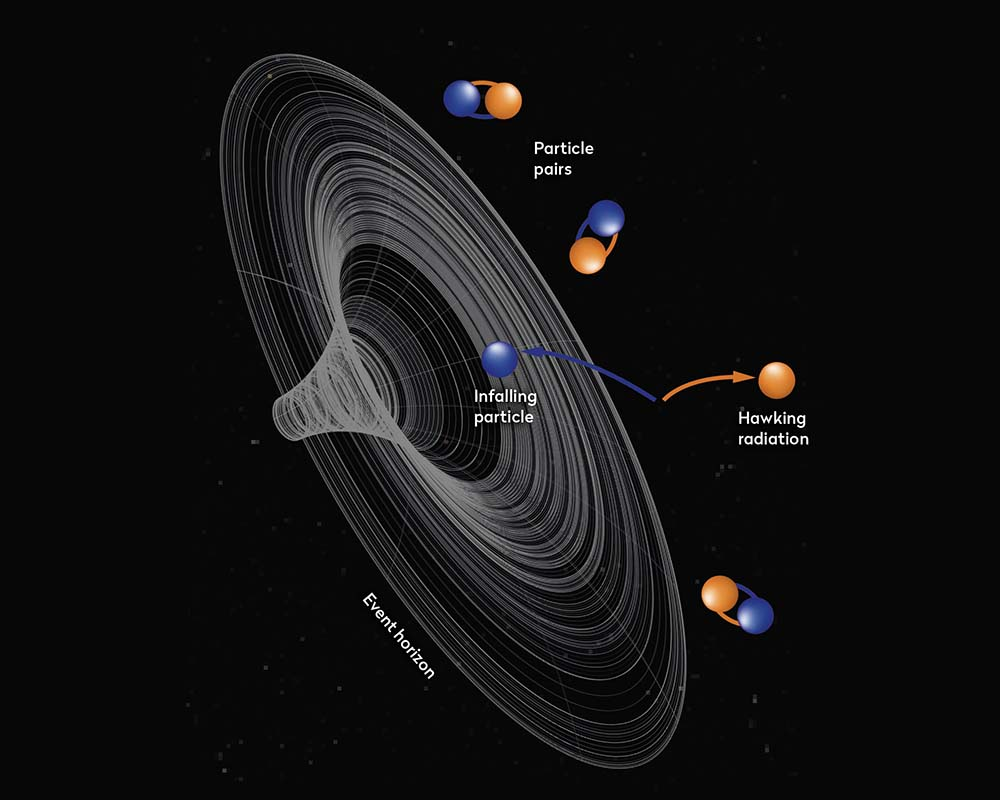
\includegraphics[width=0.8\textwidth]{47_ObserverDependentVacuum/Hawking-radiation-33a5ec1.jpg}\\
    {\small\textit{Hawking radiation}}
\end{center}